%%%%%%%%%%%%%%%%%%%%%%%%%%%%%%%%%%%%%%%%%%

\chapter{Tests of the second switcher and switcher wye on the West Beamline}\label{chap:fall2021}

%%%%%%%%%%%%%%%%%%%%%%%%%%%%%%%%%%%%%%%%%%

In 2021, the ongoing construction of the large \acrshort{msr} (Sec.~\ref{sec:MSR}) relegated the commissioning of nEDM components to the West beamline (Fig.~\ref{fig:AreaB_schematic}). Newly built second switcher and wye need to be tested.

%%%%%%%%%%%%%%%%%%%%%%%%%%%%%%%%%%%%%%%%%%%%%%

\section{Description of experimental setup (2021)}

%%%%%%%%%%%%%%%%%%%%%%%%%%%%%%%%%%%%%%%%%%%%%%

UCN tau roundhouse. A buffer volume called the ``roundhouse'' was introduced in 2018 that precleans the loaded UCNs and smooths over any temporal fluctuations in the UCN production rate while loading

New Y. NiP coated Vertical separation (center to center of beamline) $\qty{18.85}{in}\approx\qty{0.48}{m}$. Corresponds to a $\sim \qty{25}{neV}$ potential step for upper switcher and a boost to the lower switcher. 

Coils and solenoids (depicted in Fig.~\ref{subfig:west_beamline_switchers}) again keep everything under $\sim \qty{1}{mT}$ field

A second switcher had been constructed for this measurement cycle, was placed on the lower side of the switcher stand. Off this side was the single channel spin analyzer used in Chap.~\ref{chap:north_beamline_paper} and \ref{chap:lanl_ramsey_demonstration}. On the other side was a simultaneous spin analyzer (SSA)

\begin{figure}
    \centering
    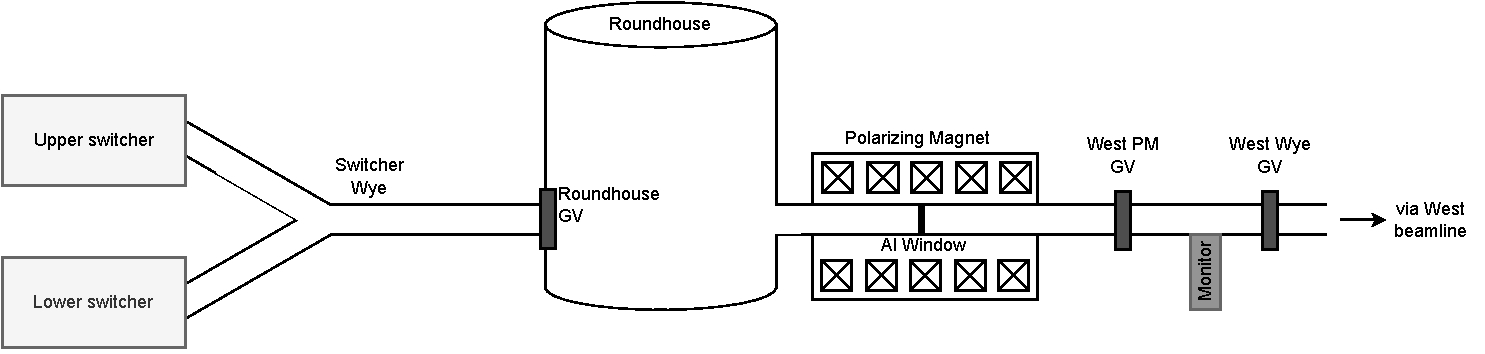
\includegraphics[width=\textwidth]{figures/westbeamline_2021.pdf}
    \caption{Caption}\label{fig:west_beamline_2021}
\end{figure}

\begin{figure}
\centering
%subfigure width gets "multiplied" by includegraphics width
\begin{subfigure}{.5\textwidth}
  \centering
  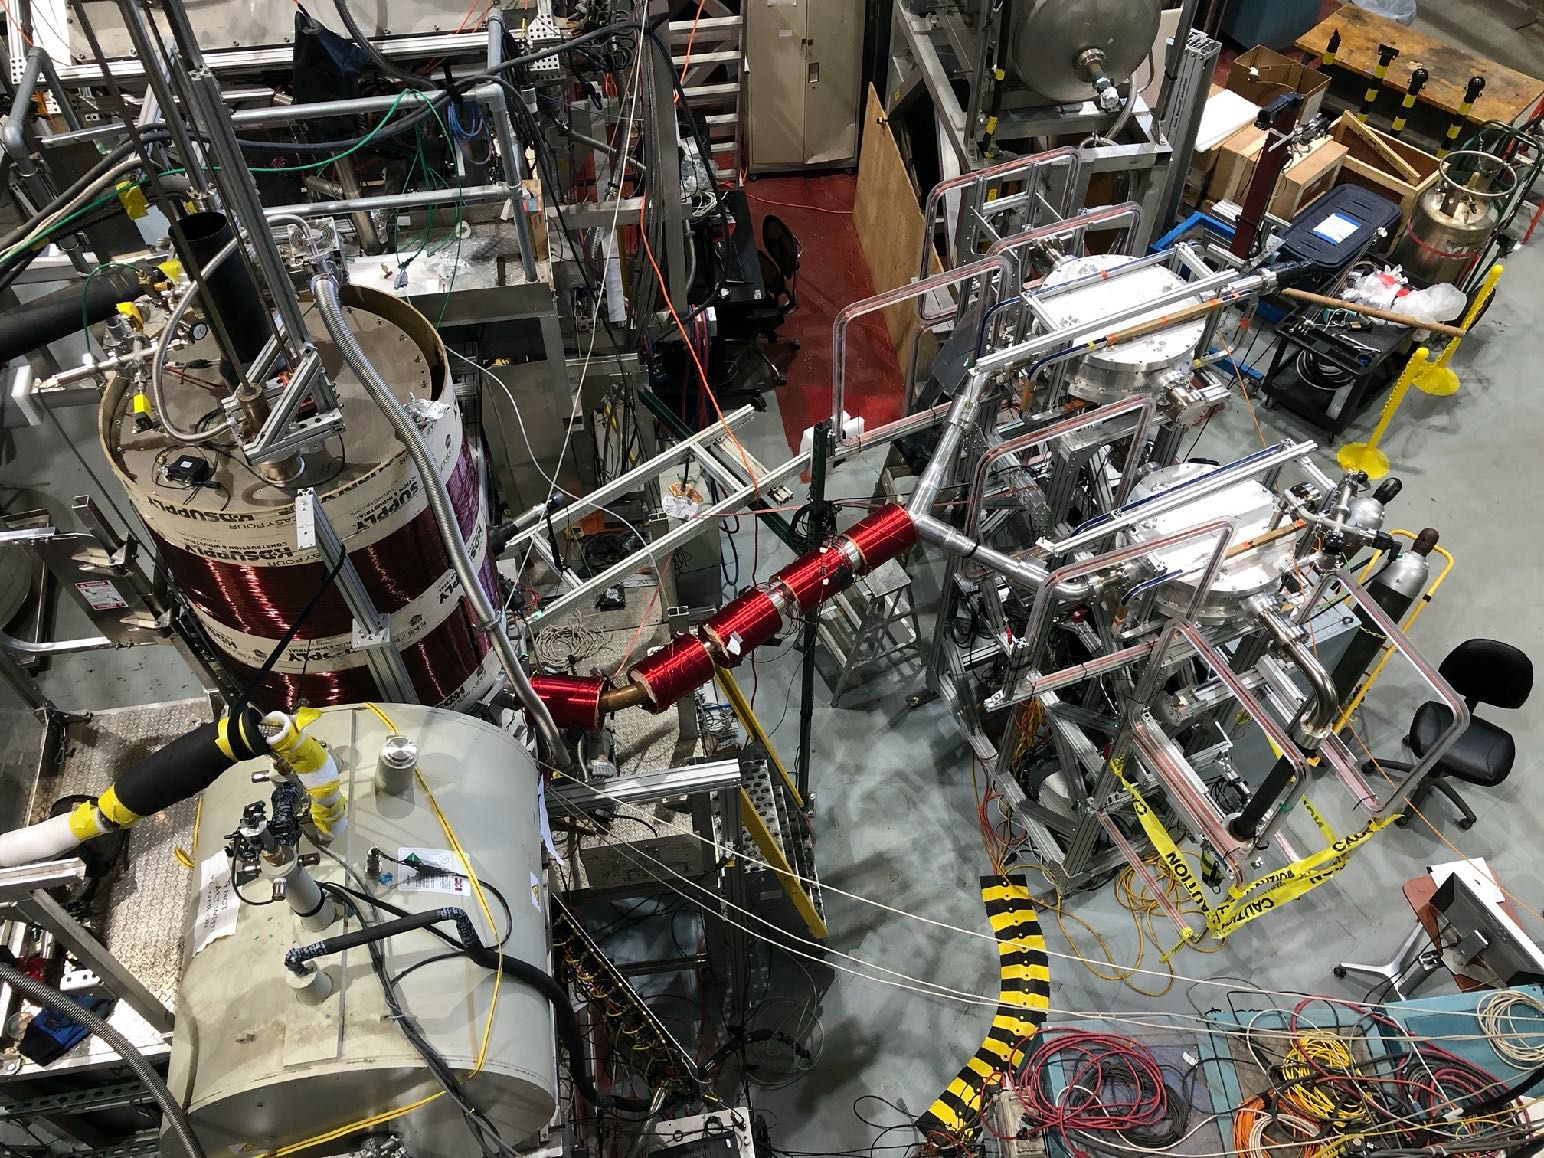
\includegraphics[width=\textwidth]{figures/west_beamline_switcher_tests.jpg}
  \vspace{5pt}
  \caption{}\label{subfig:west_beamline_switchers}
\end{subfigure}%DO NOT REMOVE THIS '%'
\begin{subfigure}{.5\textwidth}
  \centering
  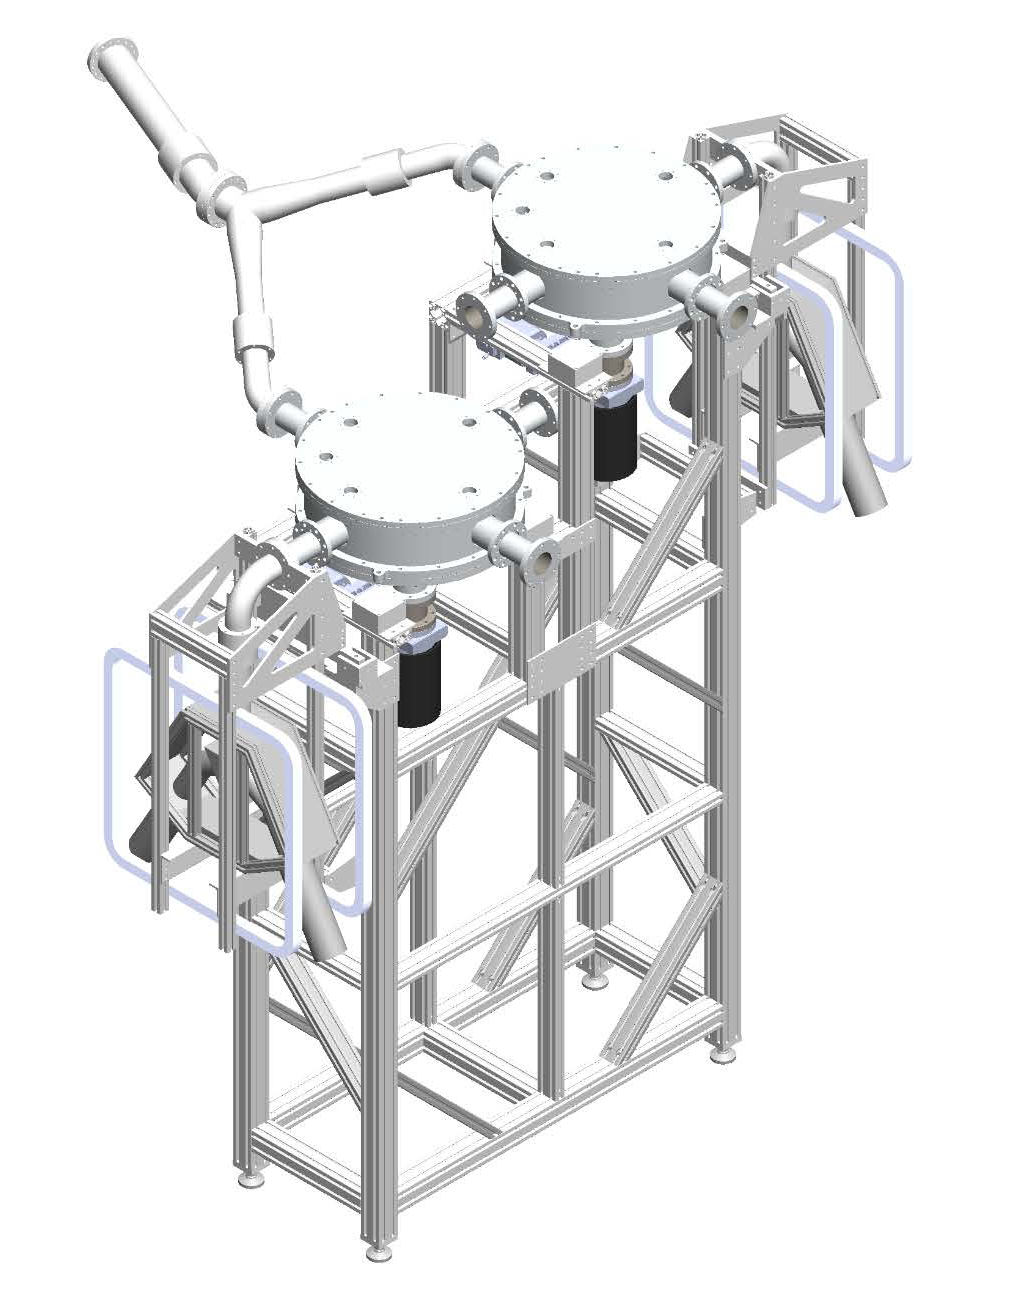
\includegraphics[height=3in]{figures/switcher_mockup.png}
  \caption{}\label{subfig:switcher_mockup}
\end{subfigure}
\caption
{Caption}
\label{fig:west_beamline_switchers}
\end{figure}



%%%%%%%%%%%%%%%%%%%%%%%%%%%%%%%%%%%%%%%%%%%%%%

\section{UCN transport measurements}

%%%%%%%%%%%%%%%%%%%%%%%%%%%%%%%%%%%%%%%%%%%%%%

\begin{figure}
\centering
%subfigure width gets "multiplied" by includegraphics width
\begin{subfigure}{.5\textwidth}
  \centering
  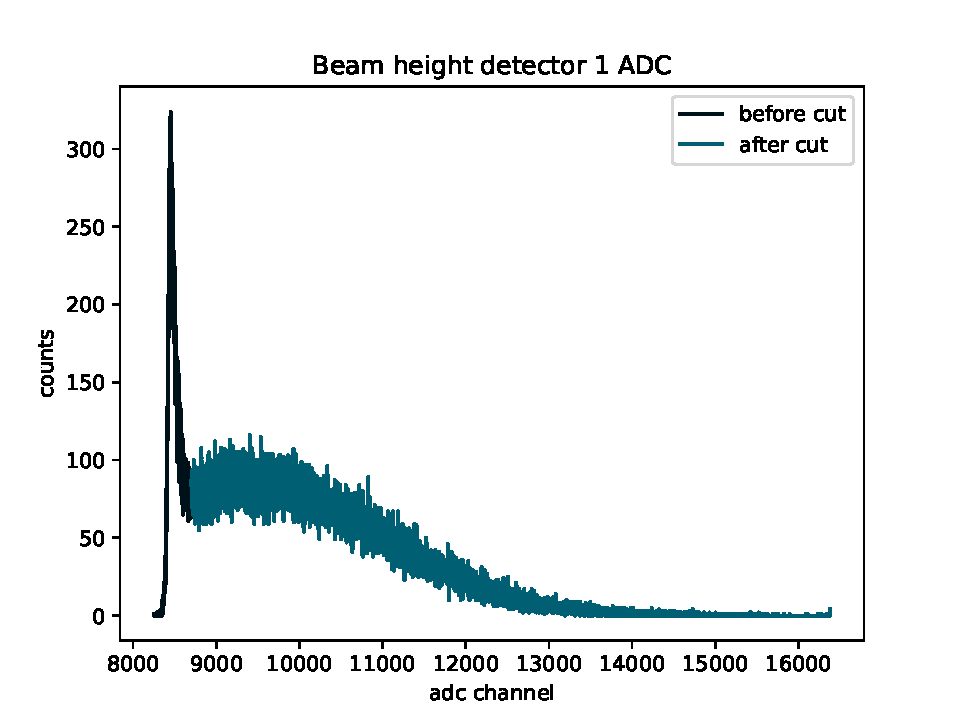
\includegraphics[width=\textwidth]{figures/2021_beam_det_1_adc.pdf}
  \caption{}\label{subfig:beam_det_1_adc}
\end{subfigure}%DO NOT REMOVE THIS '%'
\begin{subfigure}{.5\textwidth}
  \centering
  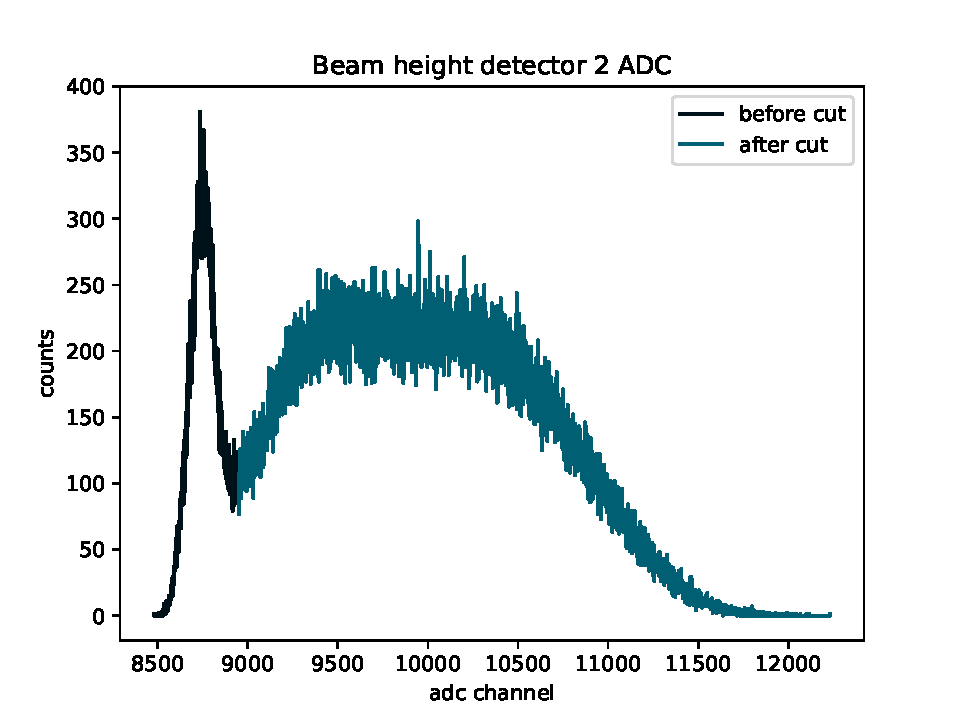
\includegraphics[width=\textwidth]{figures/2021_beam_det_2_adc.pdf}
  \caption{}\label{subfig:beam_det_2_adc}
\end{subfigure}
\begin{subfigure}{.5\textwidth}
  \centering
  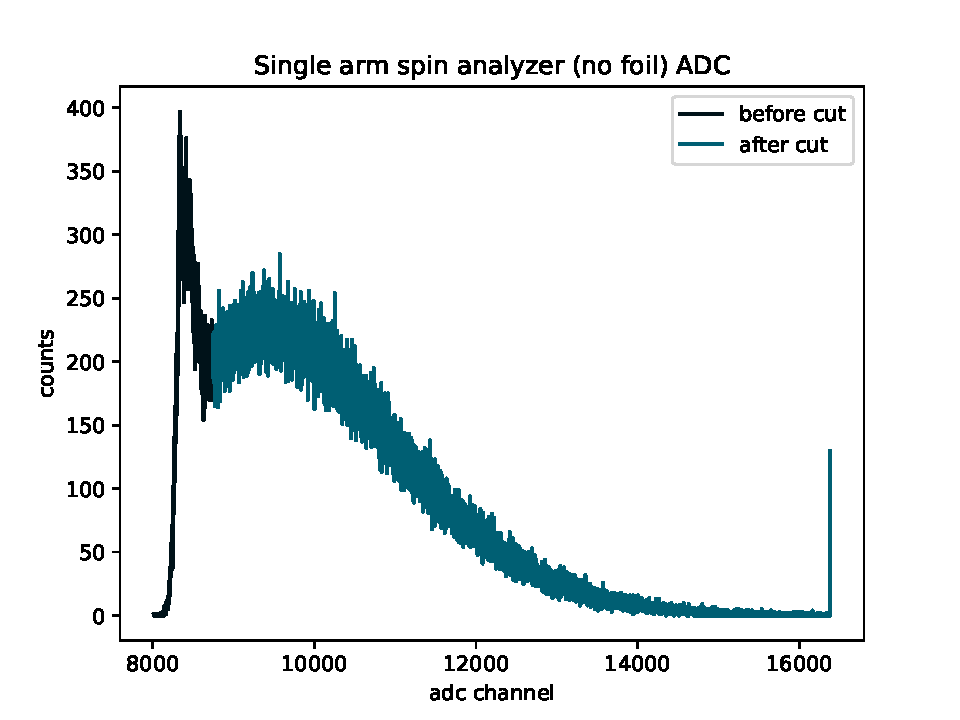
\includegraphics[width=\textwidth]{figures/2021_single_arm_no_foil_adc.pdf}
  \caption{}\label{subfig:single_arm_no_foil_adc}
\end{subfigure}
\caption
{Caption}
\label{fig:2021_detector_adc}
\end{figure}

Show ADC cuts for each detector. Spectrum did not change when detectors were moved. As is typical for the UCN spectrum from BZs we make cuts at the noise peak~\cite{jeph_multilayer_2015}

2x 3 inch BnZS scintillator (Sec.~\ref{sec:ucn_detectors})  + PMTs at beam height. 

\begin{small}
\begin{verbatim}
Both PMTs beam height on switcher 1 (higher switcher)
======================================================
SINGLE CHANNEL DET FOIL OUT
detector rate: 1443.88
wgv rate: 632.46
normalized to wgv 650 [Hz]: 1483.9230939506056

BEAM HEIGHT DET: WEST TEST PORT
detector rate: 1435.18
wgv rate: 641.26
normalized to wgv 650 [Hz]: 1454.7406668122135

BEAM HEIGHT DET: STRAIGHT THROUGH
detector rate: 1498.215
wgv rate: 635.39
normalized to wgv 650 [Hz]: 1532.6645839563103

Beam height PMTs on both switchers
======================================================
SINGLE CHANNEL DET FOIL OUT
detector rate: 1465.2666666666667
wgv rate: 656.6
normalized to wgv 650 [Hz]: 1450.5381256980404

BEAM HEIGHT DET: SWITCHER 2 (LOWER)
detector rate: 2244.225
wgv rate: 650.0416666666666
normalized to wgv 650 [Hz]: 2244.0811486443176

BEAM HEIGHT DET: SWITCHER 1 (HIGHER)
detector rate: 1512.1142857142856
wgv rate: 649.5142857142857
normalized to wgv 650 [Hz]: 1513.2450622443143

Switcher 2 transmission difference: 1.5425987599300384
\end{verbatim}
\end{small}

While a factor of 1.5 is unintuitive, PENTrack simulations indicate this is achievable in the current geometry

%%%%%%%%%%%%%%%%%%%%%%%%%%%%%%%%%%%%%%%%%%%%%%

\section{Spin asymmetry measurement with single arm spin analyzer}

%%%%%%%%%%%%%%%%%%%%%%%%%%%%%%%%%%%%%%%%%%%%%%

Single arm spin analyzer on the lower detector. Upper switcher had the SSA. 

Low contrast observed in a flow through mode measurement from the source to previously-proven the single arm detector. Need to rule out switcher depolarization! It was discovered that the roundhouse was depolarizing due to small patches of exposed stainless steel on some gate valves. 

 By comparison, a direct flow through mode measurement from the \ucn source to the spin analyzer (Fig.~\ref{fig:spin_flipper_efficiency}) gives $A(0)\approx 0.8$.


%%%%%%%%%%%%%%%%%%%%%%%%%%%%%%%%%%%%%%%%%%%%%%

\section{Roundhouse fill and unload time }

%%%%%%%%%%%%%%%%%%%%%%%%%%%%%%%%%%%%%%%%%%%%%%


\begin{figure}

\end{figure}

\begin{figure}
\centering
\begin{minipage}{.5\textwidth}
    \centering
    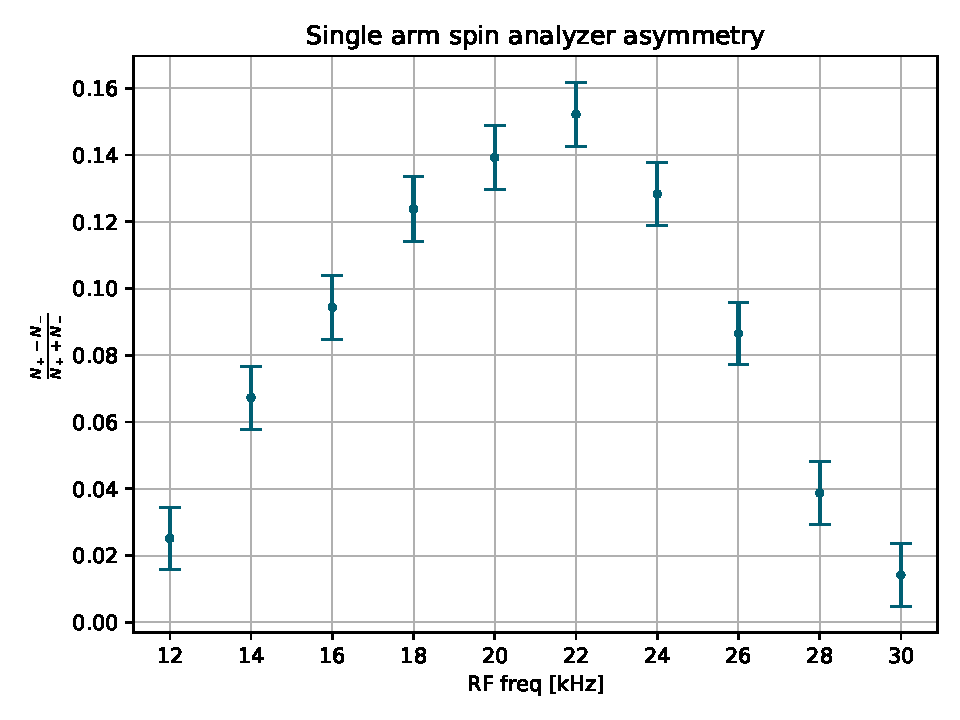
\includegraphics[width=\textwidth]{figures/single_arm_asymmetry_2021.pdf}
    \caption
    {Caption}
    \label{fig:2021_west_single_arm_asymmetry}
\end{minipage}%
\begin{minipage}{.5\textwidth}
    \centering
    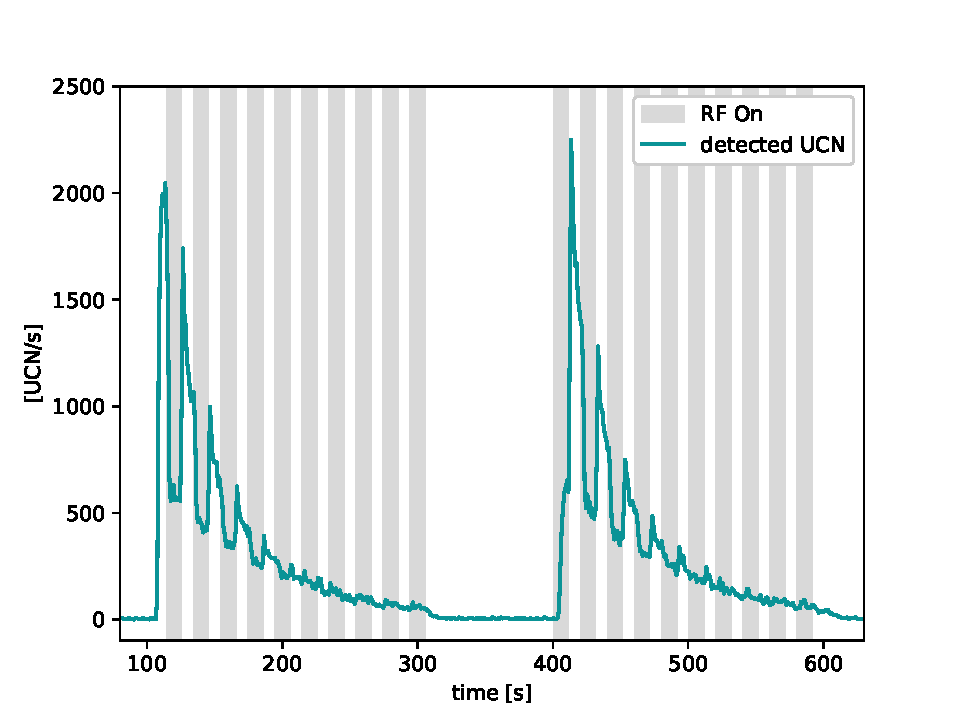
\includegraphics[width=\textwidth]{figures/2021_roundhouse_rf_toggle.pdf}
    \caption
    {Caption}
    \label{fig:roundhouse_rf_toggle_doublet}
\end{minipage}
\end{figure}

 To extract performance on the behavior of the spin analyzers, a method similar to the T1 measurement in Chap.~\ref{chap:lanl_ramsey_demonstration}. Roundhouse filling time swept. RH Gate valve was then opened. During the 200 s it took to drain the large volume of the RH, spin flipper was toggling every 10 seconds

 \begin{figure}
    \centering
    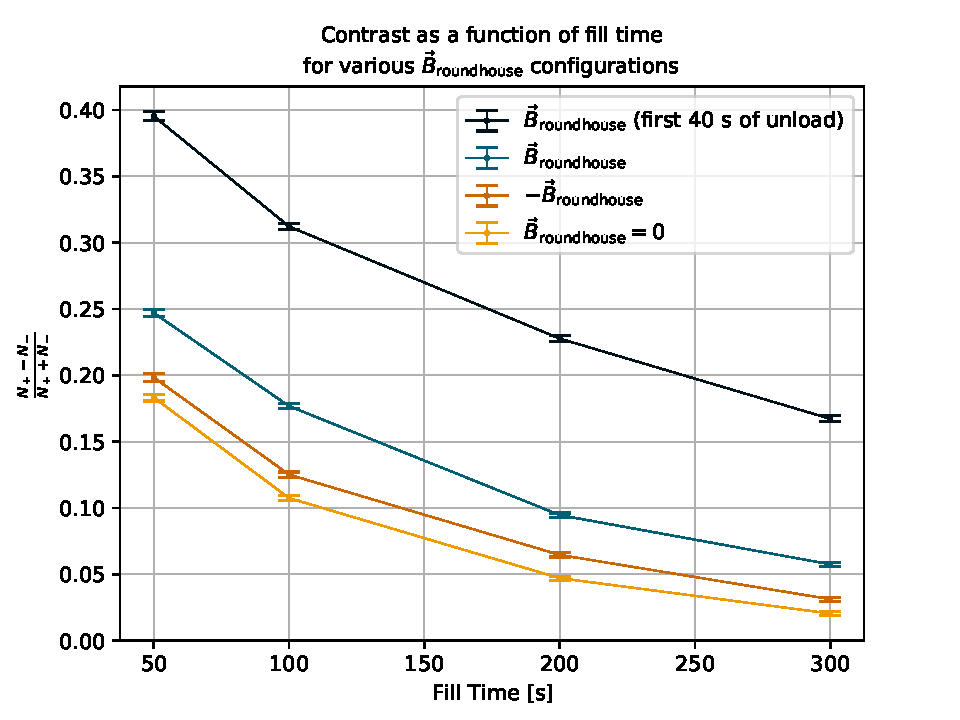
\includegraphics[width=0.7\textwidth]{figures/2021_roundhouse_asymmetry_1.pdf}
    \caption{Caption}\label{fig:2021_roundhouse_asymmetry_1}
\end{figure}

\begin{figure}
    \centering
    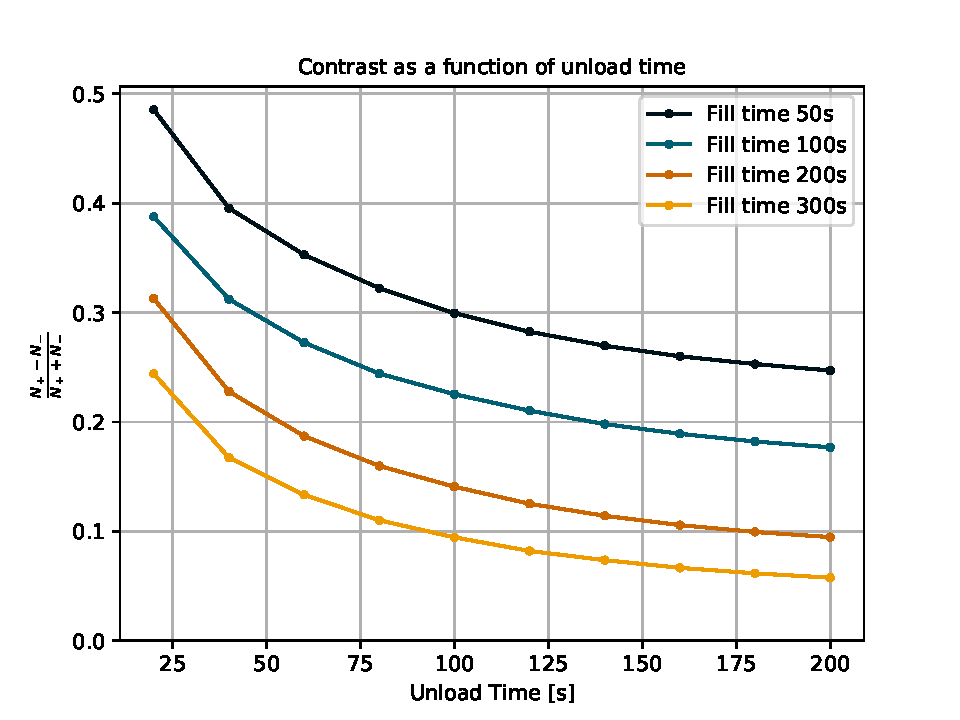
\includegraphics[width=0.7\textwidth]{figures/2021_roundhouse_asymmetry_2.pdf}
    \caption{Caption}\label{fig:2021_roundhouse_asymmetry_2}
\end{figure}